\chapter{Method}
\label{sec:VICDM}

\begin{figure}[t]
    \centering
        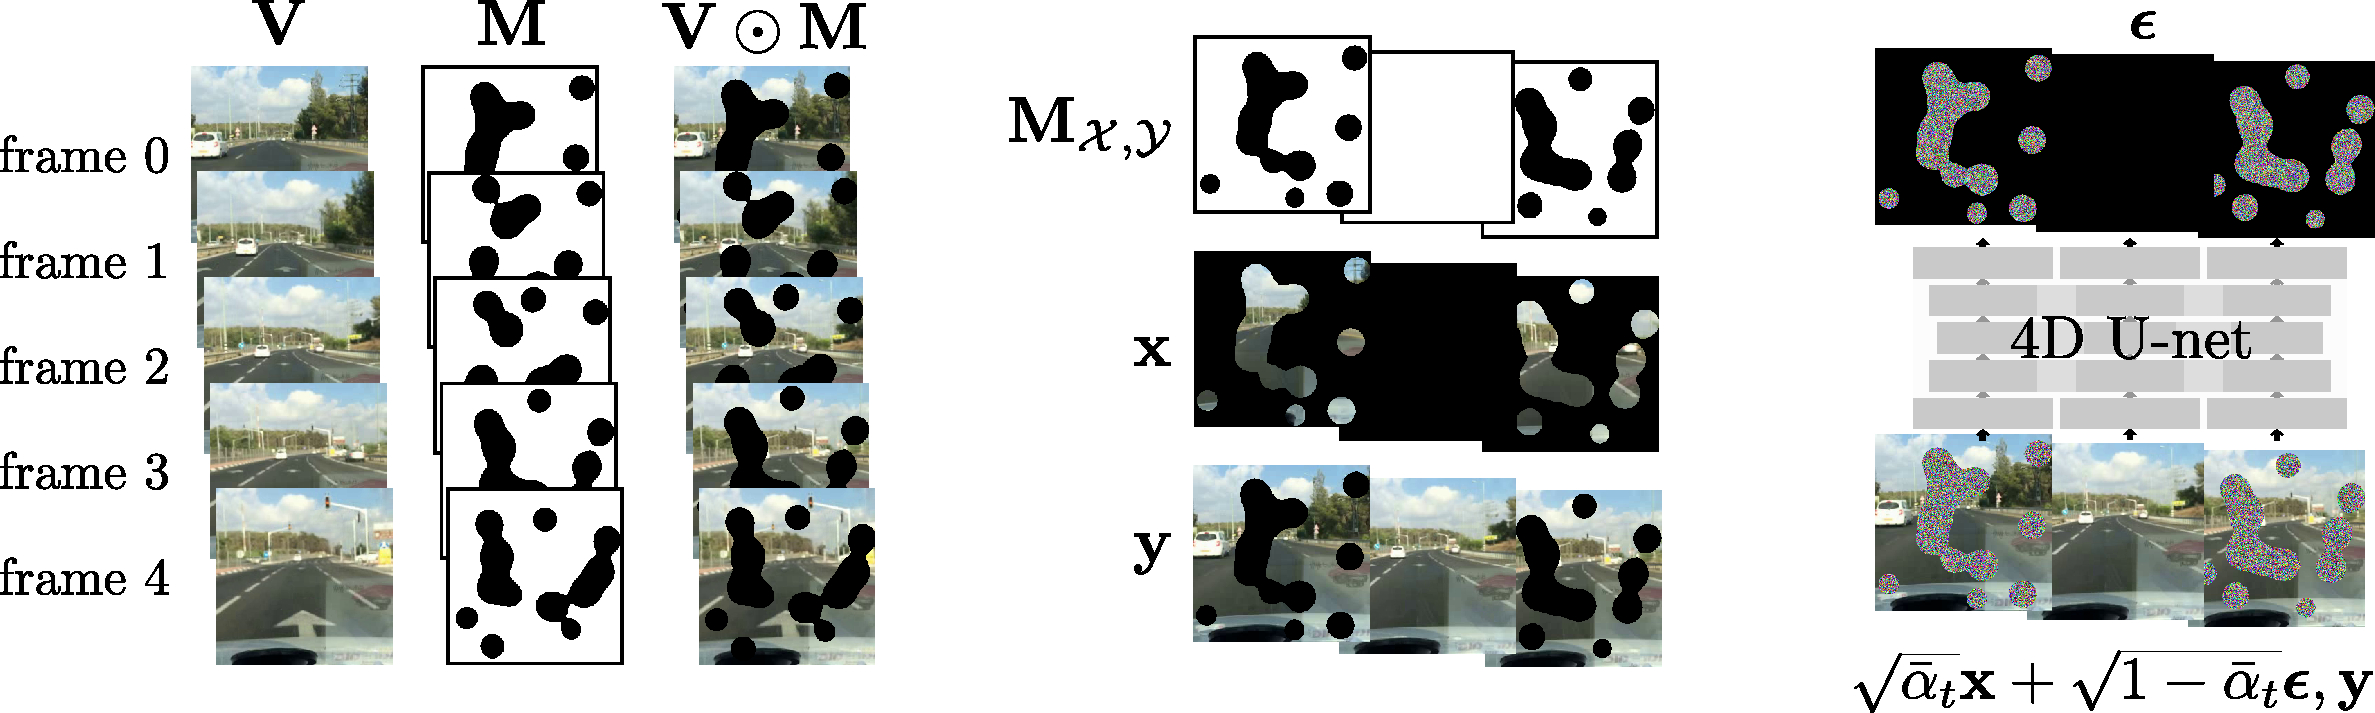
\includegraphics[width=0.9\textwidth]{figures/architecture-overview/video-inpainting-overview.pdf}
    \caption[Example model inputs during training.]{Example model inputs during training. \textbf{Left:} Visualizations of a 5-frame video $\bV$, a corresponding mask $\bM$, and the resulting known pixel values $\bV\odot\bM$. \textbf{Center:} Collated training inputs if $\fX = [0, 3]$ and $\fY = [2]$. The observations in $\by$ are then the whole of frame 2 and known pixel values in frames 0 and 3. The task is to predict the unknown pixel values in frames 0 and 3. \textbf{Right:} Inputs fed to the neural network, with noise added to pixel values in $\mathbf{x}$ but not those in $\mathbf{y}$. The task is then to predict the noise $\epsilon$. For simplicity we do not show inputs $t$, $\bM_{\fX,\fY}$, or $\fX\oplus\fY$.}
    \label{fig:arch-and-training}
\end{figure}

\section{Problem Formulation}
% \defeq \left[\bv_i\right]^N_{i=1}$,
% \defeq \left[\bm_i\right]^N_{i=1}$
We consider the problem of creating an $N$-frame video $\bV$ conditioned on some subset of known pixel values specified by a pixel-level mask $\bM$. Entries of $\bM$ take value $1$ where the corresponding pixel in $\bV$ is known and take $0$ elsewhere. We frame this as a conditional generative modeling problem, where we aim to learn an approximation of the posterior under the data distribution $p_\theta(\bV|\bV \odot \bM) \approx p_\text{data}(\bV|\bV \odot \bM)$, with $\odot$ defined such that $a \odot \bM$ returns the set of elements in $a$ for which the corresponding value in $\bM$ is 1.


Recall that, due to constraints from the network architecture, \citet{fdm} were restricted to conditioning on or generating at most $K$ frames at a time. In the video inpainting problem we are predicting and conditioning on pixels rather than frames, but our network architecture imposes an analogous constraint: we can only predict or condition on pixels from at most $K$ different frames at a time. We modify the definition of a sampling scheme from \citet{fdm} as follows: we again denote sampling schemes $\{\mathcal{X}_s, \mathcal{Y}_s\}_{s=1}^S$ with $\mathcal{X}_s$ and $\mathcal{Y}_s$ being collections of frame indices. Now, however, at each stage we sample values for only unknown pixels in frames indexed by $\mathcal{X}_s$, and condition on known pixel values in all frames indexed by either $\mathcal{X}_s$ or $\mathcal{Y}_s$. Referencing \Cref{fig:sampling-schemes}, in each row (stage) we show frames indexed by $\mathcal{X}_s$ in cyan and frames indexed by $\mathcal{Y}_s$ in either dark red or bright red. Frames shown in bright red contain missing pixels, which we do not wish to sample or condition on until a later sampling stage; we describe how we deal with this in \Cref{sec:future-conditioning}.


\section{Architecture}
We generalize the FDM architecture of \citet{fdm} to use pixel-level masks rather than frame-level masks, as in the image inpainting approach proposed by \citet{palette}. Concretely, every input frame is concatenated with a mask which takes value $1$ where the corresponding pixel is observed and $0$ elsewhere. The input values are clean (without added noise) for observed pixels and noisy values otherwise.



\section{Training Procedure} 
Recall that we wish to train a model that can generate plausible values for unknown pixels in frames indexed by $\mathcal{X}$, conditioned on known pixel values in frames indexed by either $\mathcal{X}$ or $\mathcal{Y}$. We simulate such tasks by first sampling a video $\bV$ and a mask $\bM$ from our dataset,  and then sampling frame indices $\mathcal{X}$ and $\mathcal{Y}$ from a ``frame index distribution'' similar to that of \citet{fdm}.\footnote{Our frame index distribution is a mixture distribution between the one used by \citet{fdm} and one which always samples $\mathcal{X}$ and $\mathcal{Y}$ so that they represent sequences of consecutive frames. We found that including these sequences of consecutive frames improved temporal coherence.}
The distribution over masks $\bM$ can be understood as reflecting the variability in the types of masks we will encounter at test-time, and the frame index distribution can be understood as reflecting our desire to be able to sample from the model using arbitrary sampling schemes. Given $\bM$, $\fX$, and $\fY$, we create a combined list of frames $\fX \oplus \fY$, where $\oplus$ denotes concatenation, and a corresponding mask $\bM_{\fX,\fY} := \bM[\fX] \oplus \mathbbm{1}[\fY]$, where $\mathbbm{1}[\mathcal{Y}]$ is a mask of all $1$'s for each frame indexed in $\mathcal{Y}$. This masks only the missing pixels in frames $\fX$ while treating all pixels in frames $\fY$ as observed (visualized in \Cref{fig:arch-and-training}).
We then extract our training targets from the video as $\bx := \bV[\fX\oplus\fY] \odot (1-\bM_{\fX,\fY})$, and our observations as $\by := \bV[\fX\oplus\fY] \odot \bM_{\fX,\fY}$.

\begin{algorithm}[t]
    \caption{Training Loop}
    \label{alg:train}
    \begin{algorithmic}[1]
    \Repeat
    \State $(\bV, \bM) \sim q(\bV, \bM)$\Comment{Sample video and mask}
    \State $(\mathcal{X}, \mathcal{Y}) \sim u(\mathcal{X}, \mathcal{Y})$\Comment{Sample training task}
    \State $t \sim \mathcal{U}(\{1 \ldots T\})$\Comment{Sample timestep}
    \State $\boldsymbol{\epsilon} \sim \mathcal{N}(\mathbf{0}, \mathbf{I})$\Comment{Sample noise}
    \State $\bM_{\mathcal{X}, \mathcal{Y}} \gets \bM [\mathcal{X}] \oplus \mathbbm{1}[\fY]$\Comment{Create training mask}
    \State $\bx \gets \bV[\fX \oplus \fY] \odot (\mathbf{1} - \bM_{\fX, \fY})$\Comment{Extract noised pixels} 
    \State $\by \gets \bV[\fX \oplus \fY] \odot \bM_{\fX, \fY}$\Comment{Extract known pixels} 
    \State Compute $\mathcal{L}_{\text{ours}}(\theta)$ and take gradient descent step\Comment{See \Cref{eq:lours}}
    \Until converged
\end{algorithmic}
\end{algorithm}

Resampling $\bV$, $\bM$, $\fX$, and $\fY$ for every training example therefore defines a distribution over $\bx$ and $\by$, which we use when estimating the expectation over them in \Cref{eq:lflexible}. Combining this method of sampling $\bx$ and $\by$ with our pixel-wise mask, we write the loss as
\begin{equation}
    \mathcal{L}_{\text{ours}}(\theta):=\mathbb{E}_{t, \mathbf{x}, \mathbf{y}, \mathcal{X}, \mathcal{Y}, \boldsymbol{\epsilon}}\left[(\mathbf{1}-\bM_{\fX,\fY})\odot\left\|\boldsymbol{\epsilon}-\boldsymbol{\epsilon}_\theta\left(\sqrt{\bar{\alpha}_t} \mathbf{x}+\sqrt{1-\bar{\alpha}_t} \boldsymbol{\epsilon}, \mathbf{y}, \bM_{\fX,\fY}, \fX\oplus\fY, t\right)\right\|^2\right],
    \label{eq:lours}
\end{equation}
where $\fX\oplus\fY$ provides information about each frame's index within $\bV$, and $\bM_{\fX,\fY}$ is the mask making explicit which pixels have known values.We note that the loss is only computed for unknown pixel locations. The full training loop is outlined in \Cref{alg:train}.




\section{Inpainting Long Videos} \label{sec:future-conditioning}
Given the architecture and training procedure we have described so far, we can use the resulting models to to implement the AR and Hierarchy-2 sampling schemes shown in \Cref{fig:ar,fig:h2} without further complication. A downside of these sampling schemes, however, is that they do not enable us to condition on frames with unknown pixel values. That is, we are not able to condition on the known pixels in a frame unless we either (a) have previously inpainted it and know all of its pixel values already, or (b) are inpainting it as we condition on it. We show in our experiments that this often leaves us unable to account for important dependencies in the context.



We therefore propose a method for conditioning on \textit{incomplete} frames. This enables the sampling schemes shown in \Cref{fig:sampling-schemes}, where we condition on the known pixels in incomplete frames, marked in red. Recall that $\bx$ denotes ``unknown pixels in frames indexed by $\fX$'' and $\by$ denotes ``known pixels in frames indexed by $\fX$ or $\fY$''. If any frames indexed by $\fY$ are incomplete then we have a third category, which we'll call $\mathbf{z}$: ``unknown pixels in frames indexed by $\fY$''.




We then wish to approximately sample $\mathbf{x} \sim p_\text{data}(\cdot | \mathbf{y})$ without requiring values of $\mathbf{z}$. We do not have a way to sample directly from an approximation of this distribution, as the diffusion model is not trained to condition on ``incomplete'' frames. We note, however, that this desired distribution is the marginal of a distribution that our diffusion model \textit{can} approximate:
\begin{equation}
    p_\text{data}(\mathbf{x}|\mathbf{y}) = \int p_\text{data}(\mathbf{x},\mathbf{z}|\mathbf{y}) \mathrm{d}\mathbf{z} \approx \int p_\theta(\mathbf{x},\mathbf{z}|\mathbf{y}) \mathrm{d}\mathbf{z}.
\end{equation}
This means that we can sample from the required approximation of $p_\text{data}(\mathbf{x}|\mathbf{y})$ by sampling from $p_\theta(\mathbf{x},\mathbf{z}|\mathbf{y})$ and then simply discarding $\mathbf{z}$.

\begin{figure}[t]
    \centering
    \begin{subfigure}[t]{0.3\textwidth}
        \centering
        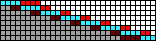
\includegraphics[width=\textwidth]{figures/sampling-scheme-visualizations/autoregressive-with-near-future.png}
        \caption{Improved AR.}
        \label{fig:improved-ar}
    \end{subfigure}
    ~
    \begin{subfigure}[t]{0.3\textwidth}
        \centering
        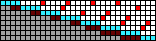
\includegraphics[width=\textwidth]{figures/sampling-scheme-visualizations/autoregressive-with-future.png}
        \caption{Improved AR w/ \\ far future.}
        \label{fig:improved-ar-w-far-future}
    \end{subfigure}
    ~
    \begin{subfigure}[t]{0.3\textwidth}
        \centering
        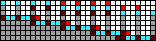
\includegraphics[width=\textwidth]{figures/sampling-scheme-visualizations/autoregressive-multires-3-1.png}
        \caption{2-res. improved AR.}
        \label{fig:multiscale}
    \end{subfigure}%
    \caption[A visualization of sampling schemes for video inpainting.]{Sampling schemes visualizations similar to \Cref{fig:old-sampling-schemes}. In addition we now also condition on observed pixel values in frames that can also contain unknown pixel values. Frames where we do so are shown in bright red and the color scheme is otherwise the same as in \Cref{fig:old-sampling-schemes}.
    }
    \label{fig:sampling-schemes}
\end{figure}

\section{Sampling Schemes}\label{sec:samplingschemes}
The ability to condition on incomplete frames enables us to design new sampling schemes that better capture dependencies that are necessary for high-quality video inpainting. \textbf{Improved AR} is a variant of AR that takes into account information from future frames by conditioning on the observed parts of the frames immediately after the sequence of frames being generated, as well as on the frames before; see \Cref{fig:improved-ar}. \textbf{Improved AR w/ Far Future} builds on ``Improved AR'' by conditioning on the observed parts of frames far in the future instead of of frames immediately after those being sampled; see \Cref{fig:improved-ar-w-far-future}.
\textbf{3-Resolution Improved AR} (3-Res. Improved AR) builds on ``Improved AR'' by first infilling every fifteenth frame using Improved AR, then infilling every fifth frame while conditioning on nearby infilled frames, and then infilling all other frames. We visualize a ``2-res.'' version (infilling every third frame and then every frame) in \Cref{fig:multiscale}. Visualizations of all sampling schemes we consider are shown in \Cref{fig:sampling-scheme-details}. 

\begin{figure}[t!]
    \centering
    \begin{subfigure}[t]{\textwidth}
        \centering
        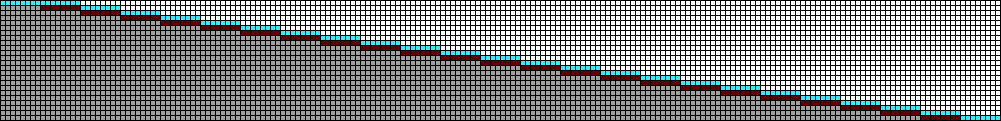
\includegraphics[width=\textwidth]{figures/big-sampling-scheme-visualizations/autoreg.png}
        \caption{AR.}
        \label{fig:ar-app}
    \end{subfigure}
    ~
    \begin{subfigure}[t]{\textwidth}
        \centering
        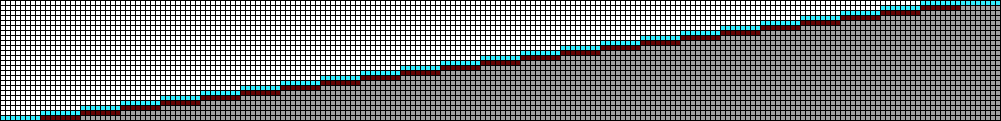
\includegraphics[width=\textwidth]{figures/big-sampling-scheme-visualizations/reverse-autoreg.png}
        \caption{Reverse AR.}
        \label{fig:reverse-ar-app}
    \end{subfigure}
    ~
    \begin{subfigure}[t]{\textwidth}
        \centering
        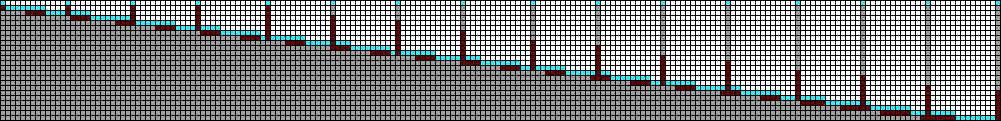
\includegraphics[width=\textwidth]{figures/big-sampling-scheme-visualizations/hierarchy-2.png}
        \caption{Hierarchy-2.}
        \label{fig:h2-app}
    \end{subfigure}
    ~
    \begin{subfigure}[t]{\textwidth}
        \centering
        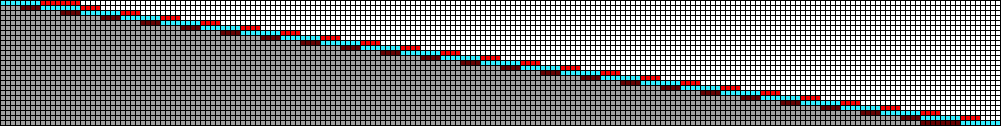
\includegraphics[width=\textwidth]{figures/big-sampling-scheme-visualizations/autoregressive-with-near-future.png}
        \caption{Improved AR.}
        \label{fig:improved-ar-app}
    \end{subfigure}
    ~
    \begin{subfigure}[t]{\textwidth}
        \centering
        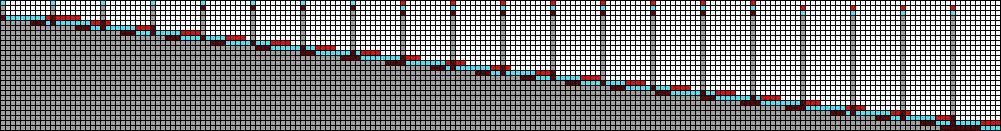
\includegraphics[width=\textwidth]{figures/big-sampling-scheme-visualizations/autoregressive-multires-10-1.png}
        \caption{2-Res Improved AR.}
        \label{fig:2res-app}
    \end{subfigure}
    ~
    \begin{subfigure}[t]{\textwidth}
        \centering
        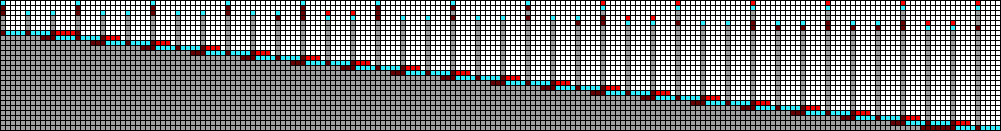
\includegraphics[width=\textwidth]{figures/big-sampling-scheme-visualizations/autoregressive-multires-15-5-1.png}
        \caption{3-Res Improved AR.}
        \label{fig:3res-app}
    \end{subfigure}
    ~
    \begin{subfigure}[t]{\textwidth}
        \centering
        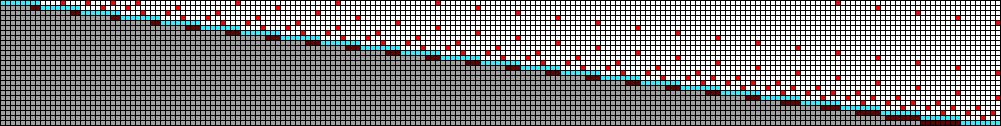
\includegraphics[width=\textwidth]{figures/big-sampling-scheme-visualizations/autoregressive-with-future.png}
        \caption{Improved AR with Far Future.}
    \end{subfigure}
    \caption[A visualization of all sampling schemes.]{Sampling schemes visualizations similar to \Cref{fig:old-sampling-schemes}, but with a model capable of attending to 16 frames at a time as in our experiments, and a more typical video length of 200.
    }
    \label{fig:sampling-scheme-details}
\end{figure}

\begin{comment}
\begin{minipage}{0.46\textwidth}
\begin{algorithm}[H]
    \centering
    \caption{Example Algorithm}\label{algorithm}
    \begin{algorithmic}[1]
\Repeat
\State $(\bV, \bM) \sim q(\bV, \bM)$\Comment{Sample video and mask}
\State $(\mathcal{X}, \mathcal{Y}) \sim u(\mathcal{X}, \mathcal{Y})$\Comment{Sample training task}
\State $t \sim \mathcal{U}(\{1 \ldots T\})$
\State $\boldsymbol{\epsilon} \sim \mathcal{N}(\mathbf{0}, \mathbf{I})$
\State $(\bV', \bM') \gets (\bV[\fX \cup \fY], \bM[\fX \cup \fY])$
\State $\bV_t' \gets \sqrt{\bar{\alpha}_t}\bV' + \sqrt{1-\bar{\alpha}_t}(\mathbbm{1}-\bM')\odot\boldsymbol{\epsilon}$
\State Take gradient descent step on \newline 
\hspace*{5em}$\nabla_\theta \|(1-\bM')\odot(\boldsymbol{\epsilon} - \boldsymbol{\epsilon}_\theta(\bV_t', \bM', \mathcal{X}, \mathcal{Y}, t))\|^2$
\Until converged
    \end{algorithmic}
\end{algorithm}
\end{minipage}
\hfill
\begin{minipage}{0.46\textwidth}
\begin{algorithm}[H]
    \centering
    \caption{Example Algorithm}\label{algorithm1}
    \begin{algorithmic}[1]
\For{$s \gets 1, \ldots, S$}
\State $\bV_s \gets \bV [\fX_s \cup \fY_s]$\Comment{Extract video frames}
\State $\bM_s \gets \bM [\fX_s \cup \fY_s]$\Comment{Extract mask frames}
\State $\hat{\bV}_s \sim \texttt{DDPM}(\cdot;\bV_s, \bM_s, \theta)$\Comment{Sample}
\State $\bV [\fX_s \cup \fY_s] \gets \hat{\bV}_s$\Comment{Insert completed frames}
\State $\bM [\fX_s] \gets \mathbbm{1}$\Comment{Update masks for inpainted frames}
\EndFor
\State \Return $\bV$
    \end{algorithmic}
\end{algorithm}
\end{minipage}


\begin{algorithm}[t]
\caption{Inpaint a video $\bV$ given binary mask $\bM$ and sampling scheme $\left[(\mathcal{X}_s, \mathcal{Y}_s)\right]^S_{s=1}$}
\label{alg:alg}
\begin{algorithmic}[1]
\Procedure{InpaintVideo}{$\bV, \bM; \theta$}
\For{$s \gets 1, \ldots, S$}
\State $\bV_s \gets \bV [\fX_s \cup \fY_s]$\Comment{Extract video frames}
\State $\bM_s \gets \bM [\fX_s \cup \fY_s]$\Comment{Extract mask frames}
\State $\hat{\bV}_s \sim \texttt{DDPM}(\cdot;\bV_s, \bM_s, \theta)$\Comment{Sample}
\State $\bV [\fX_s \cup \fY_s] \gets \hat{\bV}_s$\Comment{Insert completed frames}
\State $\bM [\fX_s] \gets \mathbbm{1}$\Comment{Update masks for inpainted frames}
\EndFor
\State \Return $\bV$
\EndProcedure
\end{algorithmic}
\end{algorithm}
\end{comment}

